\documentclass[a4paper, 10pt]{article}
\usepackage[margin=1.5in]{geometry}
\usepackage[utf8]{inputenc}
\usepackage[hidelinks]{hyperref}
\usepackage{biblatex}
\usepackage{amsthm}
\usepackage{tikz}
\usepackage{xcolor}
\usepackage{amsmath}
\usepackage{array}
\usepackage{float}
\usepackage{changepage}
\usepackage[printonlyused,withpage]{acronym}
\usepackage{scalerel,stackengine}
\usepackage{amssymb}
\usepackage{algorithm}
\usepackage{algpseudocode}
\usetikzlibrary{trees, shapes.geometric, arrows, fit}
\tikzstyle{host} = [rectangle, minimum width=1cm, minimum height=1cm, text width=3.5cm, draw=black]
\tikzstyle{arrow} = [thick,->,>=stealth, red]
\bibliography{references.bib}
\addbibresource{references.bib}
\theoremstyle{definition}
\newtheorem{definition}{Def}[section]
\def\apeqA{\SavedStyle\sim}
\def\apeq{\setstackgap{L}{\dimexpr.5pt+1.5\LMpt}\ensurestackMath{%
  \ThisStyle{\mathrel{\Centerstack{{\apeqA} {\apeqA} {\apeqA}}}}}}

% \title{IY5512 Summative CW}
% \author{Joshua Limbrey}
% \date{January 2022}

\begin{document}

\begin{titlepage}
    \begin{center}
        \Large
        \textbf{2208636}

        \vspace{5cm}
        \huge
        \textbf{Cryptanalysis of Lattice Based Post-Quantum Encryption Schemes}


        \vspace{3cm}
        


        \large
        Submitted as part of the requirements for the award of the\\MSc in Information Security\\at Royal Holloway, University of London.

        \vspace{1cm}


        
\includegraphics[width = 0.25\textwidth]{Royal_Holloway_College,_University_of_London-3251331149.jpg}

        
        \vspace{1cm}
        Information Security Group\\Royal Holloway, University of London\\August 2022



    \end{center}
\end{titlepage}

\tableofcontents

\newpage

\section{Preliminaries}

\subsection{Abbreviations and Acronyms
}
\begin{acronym}
    \acro{BDD}{bounded distance decoding}
    \acro{BKZ}{Block Korkine-Zolotarev, Schnorr and Euchner, 1994}
    \acro{CCA}{chosen ciphertext attack}
    \acro{CCA2}{adaptive chosen ciphertext attack}
    \acro{CPA}{chosen plaintext attack}
    \acro{CVP}{closest vector problem}
    \acro{FFT}{fast fourier transform}
    \acro{IND}{indistinguishability of ciphertexts}
    \acro{KEM}{key encapsulation mechanism}
    \acro{LLL}{Lenstra, Lenstra and Lov\'asz, 1982}
    \acro{LWE}{learning with errors}
    \acro{LWR}{learning with rounding}
    \acro{MLWE}{module learning with errors}
    \acro{NIST}{National Institute of Standards and Technology}
    \acro{NTT}{number theoretic transform}
    \acro{PKE}{public-key encryption}
    \acro{SVP}{shortest vector problem}
\end{acronym}

\newpage

\begin{abstract}

 Many post-quantum encryption schemes rely on the hardness of the \ac{LWE} problem as the foundational building block for the schemes. This work aims to discuss the conjectured hardness of the \ac{LWE} problem with an angle towards the NIST nominated scheme \textsc{Kyber}, looking at both the primal and dual attacks to solve lattice-based problems - with a specific interest towards the tailored improvements presented by MATZOV. The work aims to present a comprehensive and rigorous definition of lattice reduction algorithms (BKZ, LLL), lattice attacks (primal and (improved) dual attacks), and encryption schemes (\textsc{Kyber}), as well as the mathematical backgrounds of these concepts before discussing open questions uncovered during the discussion of said topics whilst raising our own for further debate.

\end{abstract}

\subsection{Introduction}
Since Regev detailed the \ac{LWE} problem \cite{10.1145/1060590.1060603}, many \ac{PKE} schemes have relied on the hardness of the worst-case lattice problem reductions to average-case \ac{LWE} for secure and efficient cryptography. Interest in this area has grown due to lattice problems' conjectured resilience to quantum computers, in light of Shor's proof of the weaknesses of classical cryptographic primitives \cite{365700}. The latest efforts in light of this work as well as that in furthering quantum computing has prompted a call for proposals for standardisation by the \ac{NIST} of post-quantum cryptographic algorithms \cite{NIST}. 

In this work, we shall detail both the \ac{LWE} and the lattice problems it relies upon for its believed hardness, before understanding the current attacks and their applications to candidates for standardisation, with the goal of introducing new readers to modern post-quantum cryptography, discussing open questions and presenting new ones, hopefully for further research.

\subsection{Definitions}

\begin{definition}[\ac{PKE} Scheme]
    Let $\Sigma$ be a \ac{PKE} scheme, consisting of the following three algorithms:
    \begin{itemize}
        \item $KeyGen$\\ \textbf{Output}: $(pk, sk)$, where $pk$ is the public key and $sk$, the private key.
        \item $Enc$\\ \textbf{Input}: $pk$ and $m$, where $pk$ is as defined above and $m$ is the plaintext message to be encrypted. \\
        \textbf{Output}: $c$, the ciphertext.
        \item $Dec$\\ \textbf{Input}: $sk$ and $c$ as defined above.\\
        \textbf{Output}: $m$, the plaintext.
    \end{itemize}
    $\Sigma$ must also satisfy a correctness condition:
    \[\forall m \in \mathcal{M} \text{ and } \forall (pk, sk) \leftarrow \Sigma .KeyGen\]
    \[\Sigma .Dec_{sk}(\Sigma .Enc_{pk}(m)) = m\]
    (with probability 1 over the randomness of $Enc$)
\end{definition}

\textbf{Note:} All security properties discussed will be for \ac{PKE} schemes.

% \begin{definition}[Indistinguishable]
%     \[(pk, sk) \leftarrow \Sigma.KeyGen \]
%     An adversary $\mathcal{A}$ produces two messages $m_0, m_1 \in \mathcal{M}$ (of equal length).
%     We choose a bit $b \in \{0,1\}$.
%     \[c = \Sigma .Enc_{pk}(m_b)\] 
%     Give the adversary $(c, pk)$, and allow them to generate a bit $a \in \{ 0,1\}$. If $a=b$, then the adversary has succeeded.\\
%     We say an encryption scheme $\Sigma$ is indistinguishable if the following holds:
%     \[\mathbb{P}(\mathcal{A} \text{ succeeds}) = \frac{1}{2} + \varepsilon \text{\qquad where $\varepsilon $ is negligible.}\] 
%     Intuitively, an encryption scheme has indistinguishability if an adversary is given a challenge ciphertext $c$, they cannot tell if it is from $m_0$ or $m_1$.
% \end{definition}
\begin{definition}[\ac{CPA} security, \ac{IND}-\ac{CPA}]
    ``Indistinguishability of ciphertexts under chosen plaintext attack" for an encryption scheme $\Sigma $.\\
    \[(pk, sk) \leftarrow \Sigma.KeyGen \]
    The adversary $\mathcal{A} $ is given $pk$ and outputs two messages $m_0, m_1$ (of equal length), and is also given a challenge ciphertext:
    \[c=\Sigma .Enc_{pk}(m_b)\text{\qquad for a chosen }b \in \{ 0,1\}.\] 
    $\mathcal{A}$ now generates a bit $a \in \{ 0,1\}$, and if $a=b$ then $\mathcal{A}$ has succeeded.\\
    The encryption scheme has \ac{CPA} security if:
    \[\mathbb{P} (\mathcal{A} \text{ succeeds}) = \frac{1}{2} + \varepsilon\text{\qquad where $\varepsilon$ is negligible.}\]
    This can intuitively be thought of as if an attacker is given access to the public key (therefore able to encrypt plaintext's of their choice \textbf{but not decrypt}), then if given the encryption of one of two plaintexts, the attacker has negligible advantage over guessing.
\end{definition}
\begin{definition}[\ac{CCA} security, \ac{IND}-\ac{CCA}]
    ``Indistinguishability of ciphertexts under a chosen ciphertext attack" for an encryption scheme $\Sigma $.\\
    \[(pk, sk) \leftarrow \Sigma.KeyGen \]
    The adversary $\mathcal{A} $ is given $pk$ and a decryption oracle $\mathcal{O}_{\Sigma .Dec_{sk}}$, and outputs $m_0, m_1$ (of equal length). The adversary is only able to query this oracle up until it receives the challenge ciphertext,
    \[c=\Sigma .Enc_{pk}(m_b)\text{\qquad for a chosen }b \in \{ 0,1\}.\] 
    $\mathcal{A} $ then generates a bit $a \in \{ 0, 1\}$, and if $a=b$ then $\mathcal{A} $ has succeeded.
    The encryption scheme has \ac{CCA} security if:
    \[\mathbb{P} (\mathcal{A} \text{ succeeds}) = \frac{1}{2} + \varepsilon \text{\qquad where $\varepsilon$ is negligible.}\]
    Intuitively, this is if an adversary is able to ask for decryptions before given the challenge, once given the challenge ciphertext they have negligible advantage over guessing.
\end{definition}
\begin{definition}[\ac{CCA2} security, \ac{IND}-\ac{CCA2}]
    ``Indistinguishability of ciphertexts under an adaptive chosen ciphertext attack" for an encryption scheme $\Sigma $.\\
    \[(pk, sk) \leftarrow \Sigma.KeyGen \]
    The adversary $\mathcal{A} $ is given $pk$ and a decryption oracle $\mathcal{O}_{Dec_{sk}}$, and outputs $m_0, m_1$ (of equal length). The adversary then receives the challenge ciphertext,
    \[c=\Sigma .Enc_{pk}(m_b)\text{\qquad for a chosen }b \in \{ 0,1\}.\]
    but may continue to query $\mathcal{O}_{Dec_{sk}}$ provided the requested decryption is not of $c$.
    $\mathcal{A} $ then generates a bit $a \in \{ 0, 1\}$, and if $a=b$ then $\mathcal{A} $ has succeeded.
    The encryption scheme has \ac{CCA2} security if:
    \[\mathbb{P} (\mathcal{A} \text{ succeeds}) = \frac{1}{2} + \varepsilon \text{\qquad where $\varepsilon$ is negligible.}\]
    Intuitively, this can be thought of as if an adversary has the ability to decrypt any ciphertext of their choice, other than the challenge; the adversary still does not have enough information to decrypt the challenge.
\end{definition}

\subsection{Notation}


We shall use $\mathcal{B} $ to denote the set of 8-bit unsigned integers (or bytes), ie. the set $\{0, ..., 255\}$. Reals and integers will be denoted by lowercase letters, distributions and sets by capital letters. Bold letters denote vectors (lower case)\footnote{with $0$ denoting the zero vector.} or matrices (capital), with the $i$th element of a vector $\mathbf{v}$ being denoted by $\mathbf{v}_i$, and the $j$th column of a matrix $\mathbf{M}$ by $\mathbf{m}_j$. $\mathbf{M}[i][j]$ denotes the entry in row $i$ and column $j$ (all vectors will be column vectors unless otherwise stated). Let the concatenation of two (row) vectors $\mathbf{v, w}$ be denoted by $(\mathbf{v} || \mathbf{w})$.

\begin{definition}[Linearly independent]
    The set of vectors $\{\textbf{v}_1,...,\textbf{v}_m\}$ are linearly independent if $\Sigma_{i=1}^m \lambda _i \mathbf{v}_i = 0$ only has the trivial solution, $\lambda _1 = ... = \lambda _m = 0$.
\end{definition}

\begin{definition}[Span]
    Let the span of a set of vectors $\{\textbf{v}_1,...,\textbf{v}_m\}$ be the set of all linear combinations $\Sigma_{i=1}^m \lambda _i \mathbf{v}_i$, where $\lambda _i \in \mathbb{R}$
\end{definition}

\begin{definition}[Inner product and norm]
    Let $\mathbf{v}, \mathbf{w} \in \mathbb{R}^n$. The inner product of $\mathbf{v}$ and $\mathbf{w}$, $\langle \mathbf{v}, \mathbf{w} \rangle = \Sigma_{i=1}^n \mathbf{v}_i \mathbf{w}_i$ and the norm of $\mathbf{v}$, $|\mathbf{v}| = \sqrt{\langle \mathbf{v}, \mathbf{v} \rangle}$.
\end{definition}

\subsubsection{Lattices}

Let $\mathbf{B} \in \mathbb{R} ^{d\times m}$ where the columns, $\mathbf{b}_i$, are linearly independent basis vectors\footnote{We will assume that $d=m$ unless otherwise stated.}. This can also be thought of as a set $\mathbf{B}=\{\mathbf{b}_1,...,\mathbf{b}_m\}\subset \mathbb{R} ^d$, where as before, $\mathbf{b}_i$ are linearly independent basis vectors. The lattice generated by $\mathbf{B}$ is defined as $\mathcal{L} = \mathcal{L} (\mathbf{B}) := \{\mathbf{B} \mathbf{x} | \mathbf{x} \in \mathbb{Z} ^d\}$. We say $Vol(\mathcal{L}) = \sqrt{\det(\mathbf{B} \mathbf{B}^T)}$.


\begin{definition}[Shortest Vector Problem, SVP]
    Given a lattice $\mathcal{L}$ with basis matrix $\textbf{B}$, find a non-zero vector $\mathbf{v} \in \mathcal{L}$ such that the length, $|\mathbf{v}|$, is minimal.

    $\lambda_i(\mathcal{L})=\min \{\max \{|\mathbf{x}_1|,...,|\mathbf{x}_i|\} : \mathbf{x}_1,...,\mathbf{x}_i \in \mathcal{L} \mbox{ are lineraly independent}\}$ - in other words, $\lambda_1(\mathcal{L})$ is the shortest non-zero vector in $\mathcal{L}$.
\end{definition}

\begin{definition}[Closest Vector Problem, CVP]
    Given a lattice $\mathcal{L}$ with basis matrix $\textbf{B}$, and a vector $\mathbf{v} \in \mathbb{R}^n$, find a vector $\mathbf{w} \in \mathcal{L}$ such that $|\mathbf{v} - \mathbf{w}|$ is minimal.
\end{definition}

\begin{definition}[Bounded Distance Decoding, BDD]
    Given a lattice $\mathcal{L}$ with basis matrix $\textbf{B}$, and a vector $\mathbf{v} \in \mathbb{R}^n$ such that its distance from the lattice is at most $(\min\{ |\mathbf{w}| : \mathbf{w}\in \mathcal{L}\backslash \{\mathbf{0}\}\})/2$, find the closest vector $\mathbf{w}\in \mathcal{L}$ to $\mathbf{v}$. In other words, given a vector such that its distance from any lattice point is less than half the shortest vector of the lattice, find the closest vector to that given.
\end{definition}




\subsection{Standard Algorithms}

\begin{definition}[\ac{FFT}]
    Given $f:G \rightarrow \mathbb{C}$ where $G$ is an abelian group, \ac{FFT} will evaluate $\hat{f}(\chi):=\Sigma _{g \in G}f(g)\chi (g)$ for all $\chi \in \hat{G}$ where $\hat{G}$ is the dual group of $G$. $\hat{G}$ is defined as the set of all homomorphisms from $G$ into the multiplicative group of roots of unity in $\mathbb{C}$. 
    
    For $f:(\mathbb{Z}/q\mathbb{Z})^n \rightarrow \mathbb{C}$, the Fourier transform is $\hat{f}(\mathbf{v}) = \Sigma _\mathbf{u} e^{\frac{2 \pi i}{q}\mathbf{v}^T\mathbf{u}}f(\mathbf{u})$.
\end{definition}

\begin{definition}[\ac{LLL} \cite{article}]
    Let $\mathbf{B}$ be the basis matrix for a lattice $\mathcal{L}$, with the corresponding Gram-Schmidt orthogonal basis matrix $\mathbf{B}^*$. This is found by first computing the Gram-Schmidt coefficients 
    
    \[\mu _{ij}=\frac{\langle \mathbf{b}_i,\mathbf{b}^*_j\rangle}{\langle\mathbf{b}^*_j,\mathbf{b}^*_j\rangle} \mbox{\qquad , $1 \leq j \leq i \leq n$}\] 
    
    and set
    
    \[\mathbf{b}^*_i=\mathbf{b}_i-\sum_{j=1}^{i-1} \mu _{i,j}\mathbf{b}^*_j\]
    with $\mathbf{b}^*_1=\mathbf{b}_1$. Then $\mathbf{B}$ is $\delta $-LLL-reduced if both conditions below hold.
    \begin{enumerate}
        \item $|\mu_{ij}| \leq \frac{1}{2}$ for $1 \leq j \leq i \leq n$.
        \item $|\mathbf{b}^*_i|^2 \geq (\delta  - \mu ^2_{i,i-1})|\mathbf{b}^*_{i_1}|^2$ for $2 \leq i \leq n$.
    \end{enumerate}
    This gives us algorithm \ref{alg:LLL}.
    \begin{algorithm}[h]
        \caption{\ac{LLL}}\label{alg:LLL}
        \begin{algorithmic}[1]
        \State \textbf{Input:} Lattice basis $\mathbf{B}$, $\delta \in(\frac{1}{4},1)$ a hermite constant
        \State $k=2$
        \State $\mathbf{b}^*_1=\mathbf{b}_1$
        \State $c_1 = |\mathbf{b}^*_1|^2$
        \If{$k > n$}
            \State \textbf{return} $\mathbf{B}$
        \EndIf
        \For{$k\gets(k-1),1$} \Comment Reduce $\mathbf{b}_k$ using previous $\mathbf{b}_j$'s.
            \State  $\mu _{ij}=\frac{\langle \mathbf{b}_i,\mathbf{b}^*_j\rangle}{\langle\mathbf{b}^*_j,\mathbf{b}^*_j\rangle} \mbox{\qquad , $1 \leq j \leq i \leq n$}$
            \State $\mathbf{b}_k = \mathbf{b}_k - \lceil \mu _{kj}\mathbf{b}_j \rceil$
            \State $\mathbf{b}^*_k = \mathbf{b}_k-\sum_{i=1}^{k-1} \mu _{k,i}\mathbf{b}^*_i$
            \State $c_k=|\mathbf{b}_k^*|^2$
            \State  $\mu _{ij}=\frac{\langle \mathbf{b}_i,\mathbf{b}^*_j\rangle}{\langle\mathbf{b}^*_j,\mathbf{b}^*_j\rangle} \mbox{\qquad , $1 \leq j \leq i \leq n$}$
        \EndFor
        \If{$c_k\geq(\delta  - \mu ^2_{k,k-1})c_{k-1}$}
            \State $k=k+1$
            \State \textbf{Go to line 3}
        \Else
            \State $temp = \mathbf{b}_k$
            \State $\mathbf{b}_k = \mathbf{b}_{k-1}$
            \State $\mathbf{b}_{k-1} = temp$
            \State \textbf{Go to line 3}
        \EndIf
        \end{algorithmic}
    \end{algorithm}
\end{definition}

\begin{definition}[Babai's Rounding and Nearest Plane Algorithm \cite{10.1007/BFb0023990}]
    Babai's rounding is a method used to solve \ac{CVP} for a lattice that has a good basis, where basis vectors are orthogonal or close to orthogonal. Let us have a lattice $\mathcal{L}$ with basis $\mathbf{B} = \{\mathbf{b}_1,...,\mathbf{b}_n\}$, then given a vector $\mathbf{v}\in \mathbb{R}^n$, we can express this as a unique linear combination

    \[\mathbf{w}=\sum_{i=1}^n \lambda _i \mathbf{b}_i \mbox{\qquad for } \lambda_i \in \mathbb{R}\]

    where $\{\lambda_1,...,\lambda_n\}$ can be found from $\mathbf{vB}^{-1}$. Babai's rounding then says to find the closest vector in our lattice to $\mathbf{v}$, $\mathbf{v}'$, we do the following

    \[\mathbf{v}'=\sum_{i=1}^n\left[\lambda_i\right]\mathbf{b}_i\mbox{.}\]

    Babai's second algorithm is the nearest plane algorithm which solves the same problem utilising a recursive search and hyperplanes. It is shown below:

    \begin{algorithm}[h]
        \caption{Babai's nearest plane algorithm}
        \begin{algorithmic}[1]
        \State \textbf{Input:} Reduced lattice basis $\mathbf{B} = \{\mathbf{b}_1,...,\mathbf{b}_n\}$, target vector $\mathbf{v}\in\mathbb{R}^n$
        \State $\mathbf{s} \gets \mathbf{v}$
        \For {$i\gets n, 1$}
            \State $\lambda = [\frac{\mathbf{s}\cdot \mathbf{b}^*_i}{\mathbf{b}_i^*\cdot \mathbf{b}_i^*}]$ \Comment Where $\mathbf{b}_i^*$ are the Gram-Schmidt vectors.
            \State $\mathbf{s} \gets \mathbf{s} - \lambda\mathbf{b}_i$
        \EndFor
        \State \textbf{return} $\mathbf{v}' = \mathbf{v} - \mathbf{s}$
        \end{algorithmic}
    \end{algorithm}
\end{definition}

\begin{definition}[\ac{NTT}]
    \ac{NTT} is a method that allows cheap and efficient multiplications in $R_q$, a polynomial ring. Let $g=\sum_{i=0}^{n-1}g_iX^i$ be a polynomial in $R_q$, then let
    \[NTT(g)=\hat{g}=\sum_{i=0}^{n-1}\hat{g}_iX^i \mbox{,\qquad where } \hat{g}_i = \sum_{j=0}^{n-1}\psi ^jg_j\omega ^{ij}\]
    and gives
    \[NTT(\hat{g})=g=\sum_{i=0}^{n-1}g_iX^i \mbox{,\qquad where } g_i = n^{-1}\psi ^{-i}\sum^{n-1}_{j=0}\hat{g}_j\omega ^{-ij}\]
    Note, that this is done so that both $NTT$ and $NTT^{-1}$ can be computed with very similar functions and the computation is almost identical, besides the difference in coefficient. Also, note that this allows us to easily and efficiently compute $f \dot g$, $f,g \in R_q$, using $f \dot g = NTT^-1(NTT(f)\circ NTT(g))$, where $\circ$ is pointwise multiplication. We also define the application of $NTT$ or $NTT^{-1}$ to a vector or matrix with elements in $R_q$ as $NTT$ or $NTT^{-1}$ being applied to each individual entry. $\circ$ is defined as being applied to vectors or matrices as usual multiplication but where the individual products of entries are pointwise multiplications of coefficients.
\end{definition}

\begin{definition}[\ac{BKZ} \cite{10.1007/3-540-54458-5_51}]
    \ac{BKZ} relies on utilising an \ac{SVP} oracle in order to KZ-reduce the basis of a lattice in a block-wise manner. If it can be ensured that each consecutive block of basis vectors of a lattice is KZ-reduced, then strong bounds on the first basis vector's length is more easily provable. A lattice $\mathcal{L} $ with basis $\mathbf{B}=\{\mathbf{b}_1, ..., \mathbf{b}_n\}$ and corresponding Gram-Schmidt orthognalised basis $\mathbf{B}^*$, is defined as being KZ-reduced if
    
    \[|\mathbf{b}_i^*| = \lambda_1(\pi_i(\mathcal{L})) \mbox{\qquad for all $i$}\]
    
    where $\pi_i(\mathbf{x})=\sum_{j \geq i} \frac{\langle \mathbf{x}, \mathbf{b}_j^*\rangle}{|\mathbf{b}^*_j|^2}\mathbf{b}^*_j$ is a projection function to project $\mathbf{x}$ orthogonally onto the span of $\{\mathbf{b}_i^*, ..., \mathbf{b}_n^*\}$.

    \begin{algorithm}[H]
        \caption{KZ-reduction}\label{alg:KZ}
        \begin{algorithmic}[1]
        \State \textbf{Input:} Basis $\mathbf{B}$ of $\mathcal{L}$, $\mathcal{O}$ an \ac{SVP} oracle
        \For {$i\gets 1, k$}
            \State Call $\mathcal{O}$ to find a $\mathbf{b}_i^*\in \pi_i(\mathcal{L})$ with $|\mathbf{b}_i^*|=\lambda_1(\pi_i(\mathcal{L}))$
            \State Lift  $\mathbf{b}_i^*$ into a $\mathbf{b}_i \in \mathbf{B}$ s.t. $\{\mathbf{b}_1,...\mathbf{b}_i\}$ is size reduced. \Comment To `lift' a vector in $\pi_i(\mathcal{L})$ to a lattice vector is to add the necessary amount of $\mathbf{b}_{i-1}$ as in general, before lifting, $\mathbf{b}_i^*$ is not in our lattice. Lifting in this manner ensures our basis remains size-reduced.
            \State Replace our basis vectors $\{\mathbf{b}_{i+1}, ..., \mathbf{b}_k\}$ with lattice vectors $\{\mathbf{b}_{i+1},...,\mathbf{b}_k\}$ s.t. $\{\mathbf{b}_1,...,\mathbf{b}_k\}$ is a basis for $\mathcal{L}$.
        \EndFor
        \State \textbf{return} KZ-reduced basis $\mathbf{B}$
        \end{algorithmic}
    \end{algorithm}

    With this, we can construct a further algorithm utilising KZ-reduction as a subroutine.

    \begin{algorithm}[H]
        \caption{\ac{BKZ} algorithm}\label{alg:BKZ}
        \begin{algorithmic}[1]
        \State \textbf{Input:} Basis $\mathbf{B} = \{\mathbf{b}_1,...,\mathbf{b}_d\}$ of $\mathcal{L}$, $\mathcal{O}$ an \ac{SVP} oracle for $k$ dimensions, blocksize $k$, hermite constant $\delta\in (\frac{1}{4}, 1)$
        \While{the basis changes}
            \For {$i\gets 1, d-k+1$}
                \State KZ-reduce basis $\pi_i(\mathbf{b}_i,...,\mathbf{b}_{i+k-1})$ using algorithm \ref{alg:KZ}
                \For {$j\gets 2, d$} \Comment size reducing $\mathbf{B}$
                    \For {$j\gets i-1, 1$}
                        \State $\mathbf{b}_i \gets \mathbf{b}_i - \left[ \mu _{i,j}\right] \mathbf{b}_j$ \Comment $\mu _{i,j}$ is the Gram-Schmidt coefficient.
                        \For {$k\gets1, j$}
                            \State $\mu _{i,k} \gets \mu_{i,k} - \left[\mu_{i,j}\right]\mu_{j,k}$
                        \EndFor
                    \EndFor
                \EndFor
            \EndFor
        \EndWhile
        \State \textbf{return} $\delta $-\ac{LLL}-reduced basis $\mathbf{B}$ where $|\mathbf{b}_i^*|=\lambda_1(\pi_i(\mathbf{b}_i,...,\mathbf{b}_{i+k-1}))$ for all $i\in\{1,...,d-k+1\}$.
        \end{algorithmic}
    \end{algorithm}
\end{definition}

\newpage

\section{Understanding the LWE problem}

\textsc{Kyber}.\ac{PKE} is a module \ac{LWE} based encryption scheme; relying on the hardness of the of the \ac{LWE} problem -  believed to be hard for both classical and quantum computers, first introduced by O. Regev \cite{10.1145/1060590.1060603}. Below is an informal mod $q$ set-up for the \ac{LWE} problem for a prime $q$:

\begin{enumerate}
    \item Let us chose an $n$ dimensional vector $\mathbf{s} \in \mathbb{F}^n_q$. This is our secret.
    \item Let us randomly and uniformly generate an $m\times n$ matrix $\mathbf{A} $ over $\mathbb{F}_q$ from elements in $\mathbb{F} _q$.
    \item Let us generate an $m$ dimensional vector, $\mathbf{e}$, s.t. $\mathbf{e}_i\sim \chi$ for all $i \in {1,...,m}$ independently for the distribution $\chi$ on $\mathbb{F}_q$ centred on $0$ with a small variance.
    \item Let $\mathbf{b} = \mathbf{A}\mathbf{s}+\mathbf{e}$ over $\mathbb{F}_q^m$
\end{enumerate}

Now, given $(\mathbf{A},\mathbf{b})$, find $\mathbf{s}$. Alternatively, the problem may be stated as given $(\mathbf{A},\mathbf{b})$, determine if $(\mathbf{A},\mathbf{b})$ was generated from our \ac{LWE} set-up or uniformly at random. Formally defined, this is as follows:\par

\begin{definition}[\ac{LWE}]
    Let $n,m,q \in \mathbb{N}$. Let $\chi _\mathbf{s}$, $\chi _\mathbf{e}$ be distributions over $\mathbb{Z}/q\mathbb{Z}$. Further, let $LWE_{n,m,q,\chi _\mathbf{s}, \chi _\mathbf{e}}$ be the probability distribution on $(\mathbb{Z}/q\mathbb{Z})^{m \times n} \times (\mathbb{Z}/q\mathbb{Z})^m$ from independently and uniformly sampling coordinates of $\mathbb{A} \in(\mathbb{Z}/q\mathbb{Z})^{m \times n}$ over $\mathbb{Z}/q\mathbb{Z}$, independently sampling coordinates of $\mathbf{s}\in (\mathbb{Z}/q\mathbb{Z})^n$, $\mathbf{e}\in (\mathbb{Z}/q\mathbb{Z})^m$ from $\chi _\mathbf{e}$ and $\chi _\mathbf{e}$ respectively. This outputs $(\mathbf{A},\mathbf{As} + \mathbf{e})$.

    \begin{itemize}
        \item \textbf{Decision-LWE:} Distinguish $LWE_{n,m,q,\chi _\mathbf{s}, \chi _\mathbf{e}}$ from the uniform distribution over $(\mathbb{Z}/q\mathbb{Z})^{m \times n} \times (\mathbb{Z}/q\mathbb{Z})^m$.
        \item \textbf{Search-\ac{LWE}:} Given a sample from $LWE_{n,m,q,\chi _\mathbf{s}, \chi _\mathbf{e}}$, recover $\mathbf{s}$.
    \end{itemize}
\end{definition}

This problem can be reduced to solving the lattice problems \ac{SVP}, \ac{CVP} or \ac{BDD}.\par  

\subsection{Lattices (revisited)}

For the reduction of \ac{LWE} to lattice problems, let us first consider the  $q$-ary lattice\footnote{A $q$-ary lattice generated by $\mathbf{B}\in\mathbb{Z}^{d\times n}_q$ is defined as $\mathcal{L}_q(\mathbf{B})=\{\mathbf{y}\in \mathbb{Z}^d|\mathbf{y}=\mathbf{Bz}\mod{q}, \mathbf{z}\in\mathbb{Z}^n \}$.}
\[\mathcal{L}_{Im(\mathbf{A})}=\{y \in \mathbb{Z}^m | y=\mathbf{Az}\mod{q} \mbox{ for some } \mathbf{z} \in \mathbb{Z}^n \}\]
from the image of our matrix $\mathbf{A}$, $Im(\mathbf{A})={\mathbf{A}x|x\in \mathbb{F}_q^n}$, which we can see has the volume
\[Vol(\mathcal{L}_{Im(\mathbf{A})})=q^{m-n}\text{.}\]

This lattice is generated by the column vectors of our matrix $\mathbf{A}\mod{q}$. From here, we can find our $m \times m$ basis matrix, $\textbf{B}_{Im(\textbf{A})}$ through the reduction of the $(n+m) \times m$ matrix
\[\mathbf{A}^T_q = (\frac{\mathbf{A}^T}{q\mathbf{I}_m})\]

Therefore, we can see that given $(\mathbf{A}, \mathbf{b})$ from an \ac{LWE} problem, we can use these to generate a lattice $\mathcal{L}_{Im(\mathbf{A})}$. Then by finding the closest point to $\mathbf{b} = \mathbf{As} + \mathbf{e}$, we can find $\mathbf{s}$ (the closest vector to $\mathbf{b}$ should be $\mathbf{As}$ given $\mathbf{e}$ is small enough) - solving the \ac{LWE} problem if \ac{CVP} can be solved.

% \cite{LWR}.



\section{The Dual and Primal Attacks}

Both the dual and primal attacks are approaches widely believed to the most promising in solving the hard lattice problems we have just discussed. Primal attacks rely on embedding techniques followed by lattice reductions (such as BKZ or LLL) in order to solve the posed problems, or alternatively, the use of Voronoi cells and sieving if preprocessing is possible. Dual attacks, meanwhile, utilise the dual lattice, taking short vectors and computing dot products with the target vector to gain evidence to see  whether the target vector lies close to the lattice. This is then repeated with many dual vectors, a distinguisher is constructed and gradient ascent search algorithms used to solve our problems. In this paper, we will focus on the dual attack, due to the recent advancements relative to \textsc{Kyber} \cite{matzov_2022_6412487}.

\subsection{Primal Attack}

The primal attack relies on the transformation of a search-\ac{LWE} instance into \ac{SVP}, via embedding and solving this by lattice reduction, enumeration, or sieving. Lattice reduction relies on the reduction of a lattice with basis matrix $\mathbf{B}$ to a lattice with basis vectors that are orthogonal or close to orthogonal, from which we can solve \ac{SVP} much easier. Enumeration utilises an exhaustive search of integer combinations of basis vectors to find the shortest; note that a bound of some sort must be placed else our problem becomes intractable due to an infinite number of possibilities to try. Sieving aims to reduce the high run times that enumeration suffers from, however itself comes with the problem of needing exponential space - meaning that the dimensions of the lattice we are searching must be considered when deciding what method one should use. Sieving relies on first beginning with an estimate for the shortest vector, and running the algorithm many times in order to make this estimate more accurate.

\subsubsection{Kannan's Embedding}

Kannan's embedding \cite{Kannan1987MinkowskisCB} is a method that allows the reduction of \ac{BDD} to unique-\ac{SVP}, where given an LWE instance $(\mathbf{A}, \mathbf{b} = \mathbf{As+e})$, we can embed the corresponding $q$-ary LWE lattice, $\mathcal{L}(\mathbf{A}) = \{\mathbf{y} \in \mathbb{Z}^m | \mathbf{y} = \mathbf{Az} \mod{q}, \forall \mathbf{z}\in \mathbb{Z}^n\}$, into $\mathcal{L}(\mathbf{B})$, a lattice with u\ac{SVP} structure and higher dimension, where 

\[\mathbf{B} = 
\begin{pmatrix}
    \bar{\mathbf{A}} & \mathbf{b}\\
    0 & t\\
\end{pmatrix}\]

and $\bar{\mathbf{A}}$ is the basis of the $\mathcal{L}(\mathbf{A})$. Then, if $t \leq \frac{\lambda_1(\mathcal{L}(\mathbf{A}))}{2} = \mbox{dist}(\mathbf{c}, \mathcal{L}(\mathbf{A}))$, \footnote{Where $\mbox{dist}(\mathbf{c}, \mathcal{L}(\mathbf{A}))$ is the distance from $b$ to the lattice, $|\mathbf{b} - \mathbf{v}|$ where $\mathbf{v}\in \mathcal{L}(\mathbf{A})$ is the closest lattice point to $\mathbf{b}$} then $\mathcal{L}(\mathbf{B})$ contains a unique shortest vector $\mathbf{w} = (\mathbf{e}^T || -t)$, allowing the easy recovery of the error and consequently the secret also. As such, our focus is now on solving \ac{SVP}.

\subsubsection{Lattice Reduction}

Once we have embedded the lattice properly, the first method we can use to solve \ac{LWE} is by lattice reduction. This will generally utilise \ac{LLL} or \ac{BKZ}, algorithms \ref{alg:LLL} and \ref{alg:BKZ} respectively. These algorithms will return a whole basis of short vectors, and so we can take the shortest, generally $\mathbf{b}_1$, as our solution - however this will not always be the true shortest vector and so they solve approximate \ac{SVP}. In some cases, if the approximation factor is low enough, this may be sufficient to break an encryption scheme. Alternatively, lattice reduction can be used in order to solve \ac{CVP}. 

It can be seen that both \ac{SVP} and \ac{BDD} can be reduced to the more general problem of \ac{CVP}. The reduction of \ac{BDD} is simple due to the only difference being the added condition to the input vector. However, \ac{SVP} to \ac{CVP} is not necessarily as simple, as using an oracle for \ac{CVP} with input $\mathbf{0}$ will return $\mathbf{0}$, because this is also a lattice vector. Instead, we can do the following. Let $\mathcal{L}$ be a lattice and $\mathbf{B}=\{\mathbf{b}_1,...,\mathbf{b}_m\}$ be the basis matrix, and let $\mathbf{B}^{(i)}=\{\mathbf{b}_1,...,\mathbf{b}_{i-1}, 2\mathbf{b}_{i},\mathbf{b}_{i+1},...,\mathbf{b}_m\}$. Then, for each $1 \leq i \leq m$, call our oracle for CVP with inputs $\mathbf{B}^{(i)}$ and $\mathbf{b}_i$, returning $\mathbf{x}_i$. Then, our shortest vector of $\mathcal{L}$ is $\min\{|\mathbf{x}_i - \mathbf{b}_i| : 1 \leq i \leq n\}$. As such, one may use a lattice reduction algorithm followed by Babai's rounding method or nearest plane algorithm in order to find the closest vector, and thus shortest vector also.

\subsubsection{Enumeration}

Lattice enumeration is akin to a brute force attack, however, as the number of vectors in a lattice is infintite, we must place a bound on the vectors we will enumerate ($R>0$, and $R\geq \lambda_1(\mathcal{L})$), which we then use to enumerate all vectors shorter than $R$. Generally, $R$ is chosen to be the length of our first basis vector. Again, we must reduce and orthogonalise our basis $\mathbf{B}$ to get $\mathbf{B}^*$ and choose a vector $\mathbf{v}\in\mathcal{L}$ s.t. $\lambda_1(\mathcal{L}) \leq \mathbf{v} \leq R$, for a lattice $\mathcal{L}$ of dimension $d$. Note that all basis vectors may be written as a linear combination of Gram-Schmidt vectors:
\[\mathbf{b}_i = \mathbf{b}_i^* + \sum_{j=1}^{i-1}\mu_{i,j}\mathbf{b}_j^*\]
but also that since $\mathbf{v}$ is a lattice vector, it can be expressed as a linear combination of basis vectors:
\[\mathbf{v} = \sum_{i=1}^{d}v_i\mathbf{b}_i\]
Therefore, we can rewrite $\mathbf{v}$ as
\[\sum_{i=1}^{d}v_i(\mathbf{b}_i^* + \sum_{j=1}^{i-1}\mu_{i,j}\mathbf{b}_j^*) = \sum_{j=1}^{d}(v_j + \sum_{i=j+1}^{d}v_i\mu_{i,j})\mathbf{b}_j^*\]
which also simplifies the projection of $\mathbf{v}$:
\[\pi_k(\mathbf{v}) = \pi_k(\sum_{j=1}^{d}(v_j + \sum_{i=j+1}^{d}v_i\mu_{i,j})\mathbf{b}_j^*) = \sum_{j=k}^{d}(v_j + \sum_{i=j+1}^{d}v_i\mu_{i,j})\mathbf{b}_j^*\]
and given the Gram-Schmidt vectors are orthogonal,
\[\left\lvert \sum_{j=k}^{d}(v_j + \sum_{i=j+1}^{d}v_i\mu_{i,j})\mathbf{b}_j^*\right\rvert^2= \sum_{j=k}^{d}(v_j + \sum_{i=j+1}^{d}v_i\mu_{i,j})^2|\mathbf{b}_j^*|^2\]

Note also, that the projection of a vector cannot be shorter than the vector itself, and so we can create the following inequality:

\[|\pi_k(\mathbf{v})|^2 = \sum_{j=k}^{d}(v_j + \sum_{i=j+1}^{d}v_i\mu_{i,j})^2|\mathbf{b}_j^*|^2\leq R^2 \mbox{\quad }\forall k\in\left[1,...,d\right]\]

We are now able to use this inequality for our enumeration. We begin by enumerating all vectors $\mathbf{w}\in \pi_d(\mathcal{L})$ of length at most $R$, and then for all potential candidates, enumerate all vectors in $\pi_{d-1}(\mathcal{L})$ of length at most $R$ that project to $\mathbf{v}$. This is then repeated all the way down in a recursive fashion, until all vectors in $\pi_1(\mathcal{L})$, $\mathcal{L}$, have been enumerated.

Therefore, if we try all possible linear combinations that satisfy our inequality, we can create a list of all lattice vectors shorter than $R$, and thus finding the shortest from a list is simple.

\subsubsection{Sieving}

Sieving aims to reduce the run-time of the very greedy approach of enumeration, however they also require exponential space - meaning that depending on the dimension of the lattice, they may not be the most efficient. First, we must take an estimate for the length of the  shortest vector\footnote{The true shortest vector $\lambda_1(\mathcal{L})$ is not generally known} in $\mathcal{L}$, call this $\tilde{\lambda}$. This can be increased if we find no vectors of at most this length, or decreased if our estimate was too generous.

The algorithm first must collect a list of small error vectors $\mathbf{e}_i$, and an associated lattice vector $\mathbf{v}_i$. Then, letting $\mathbf{r}_i = \mathbf{v}_i + \mathbf{e}_i$, rewrite this as a shorter vector $\mathbf{r}_i' = \mathbf{v}_i' + \mathbf{e}_i$ with $\mathbf{r}_i'$ that have already been found, and add $\mathbf{v}_i'$ to our list $Q$. This is then repeated such that we are adding vectors of norm no greater that $|\mathbf{B}|$, and at least a distance $\tilde{\lambda}$ apart pairwise. We do this until we find a $\mathbf{v},\mathbf{w}\in Q$ that are at most $\tilde{\lambda}$ distance apart, or until we run out of space. Below, is the Micciancio-Voulgaris sieving algorithm.

\begin{algorithm}[H]
    \caption{Micciancio-Voulgaris sieving algorithm \cite{inproceedings}}
    \begin{algorithmic}[1]
    \State \textbf{Input:} A reduced basis $\mathbf{B}=\{\mathbf{b}_1,...,\mathbf{b}_d\}$ of a lattice $\mathcal{L}$, and an estimate $\tilde{\lambda}$ for $\lambda_1(\mathcal{L})$.
    \State $Q \gets \emptyset$
    \State $\xi \gets 0.685$
    \State $N \gets \mbox{poly}(d)\cdot 2^{3.199d}$
    \For{$i\gets1, N$}
        \State $\mathbf{e}_i \in _R B_d(\mathbf{0}, \xi \tilde{\lambda})$
        \State $\mathbf{r}_i \gets \mathbf{e}_i \mod{B}$
        \While {$\exists \mathbf{v}_j \in Q : |\mathbf{r}_i - \mathbf{v}_j| \leq (1-\frac{1}{d})|\mathbf{v}_i|$}
            \State $\mathbf{r}_i \gets \mathbf{r}_i \mathbf{v}_j$
        \EndWhile
        \State $\mathbf{v}_i \gets \mathbf{r}_i \mathbf{e}_i$
        \If {$\mathbf{v}_i \notin Q$}
            \If {$\exists \mathbf{v}_j \in Q : |\mathbf{v}_i - \mathbf{v}_j| < \tilde{\lambda}$}
                \State \textbf{return} $\mathbf{v}_i - \mathbf{v}_j$
            \EndIf
            \State $Q \gets Q \cup \{\mathbf{v_i}\}$
        \EndIf
    \EndFor
    \end{algorithmic}
\end{algorithm}
Therefore, if we find two vectors $\mathbf{v,w}\in\mathcal{L}$ which are at most $\tilde{\lambda}$ apart, then $\mathbf{u} = \mathbf{v} - \mathbf{w}$ is also in our lattice and has length at most $\tilde{\lambda}$ and $\mathbf{u}$ is returned by the algorithm.

\subsubsection{Voronoi Cells}

\begin{definition}[(Open) Voronoi cell]
    Given a lattice $\mathcal{L}$, then the (open) Voronoi cell be the set
    \[\mathcal{V}(\mathcal{L}) = \{\mathbf{x} \in \mathbb{R}^n : \forall \mathbf{v} \in \mathcal{L} \backslash \{\mathbf{0}\}, |\mathbf{x}| < |\mathbf{x} - \mathbf{v}|\}\]
    This is the set of all points closer to the origin than any other lattice vector. The closed Voronoi cell, $\bar{\mathcal{V}}(\mathcal{L})$ is defined as the topological closure of the above set. Similarly, the Voronoi cell of a lattice point $\mathbf{w} \in \mathcal{L}$ is defined as
    \[\mathcal{V}(\mathcal{L})_{\mathbf{w}} = \{\mathbf{x} \in \mathbb{R}^n : \forall \mathbf{v} \in \mathcal{L} \backslash \{\mathbf{0}\}, |\mathbf{x} - \mathbf{w}| < |\mathbf{x} - \mathbf{v}|\}\]
    and is equal to $\mathbf{v}+\mathcal{V}(\mathcal{L})$. We also define the half-space
    \[H_{\mathbf{v}} = \{\mathbf{x} : |\mathbf{x}| < |\mathbf{x} - \mathbf{v}|\}\]
    and define the set of relevant vectors $V$ as being the minimal set of lattice vectors such that $\mathcal{V}(\mathcal{L}) = \bigcap _{\mathbf{v}\in V}H_{\mathbf{v}}$.
\end{definition}
When looking at utilising Voronoi cells to solve \ac{CVP} or \ac{SVP}, we will rely on the following equivalences:
\begin{enumerate}
    \item $\mathbf{t}_s$ is the shortest vector of the coset $\mathcal{L} + \mathbf{t}$
    \item $\mathbf{t}_s \in \mathcal{L} + \mathbf{t}\cap \mathcal{V}(\mathcal{L})$
    \item \ac{CVP}$(\mathbf{t}) = \mathbf{t} - \mathbf{t}_s$
\end{enumerate}
    
for $\mathbf{t}, \mathbf{t}_s$ vectors in the span of $\mathcal{L}$. We will also use Voronoi's theorem:

\textit{Let $\mathcal{L}$ be a lattice and $\mathbf{v}\in \mathcal{L}$ a non-zero vector. Then $\mathbf{v} \in V$ if and only if the pair $\pm \mathbf{v}$ are unique shortest vectors of the coset $2\mathcal{L} + \mathbf{v}$.}

Now, to solve \ac{CVP}, we will detail an algorithm to first solve \ac{CVP} for a special case where our target vector is an element of $2\bar{\mathcal{V}}(\mathcal{L})$, and then solving \ac{CVP} by making calls to this algorithm. This first algorithm makes use of the above equivalences and finds a shortest vector $\mathbf{t}_s \in \bar{\mathcal{V}}(\mathcal{L})\cap (\mathcal{L} + \mathbf{t})$ and outputs $\mathbf{t} - \mathbf{t}_s$, the closest lattice vector.

We first take our target vector $\mathbf{t}$ and relevant vectors $V$ of our lattice $\mathcal{L}$ as inputs and begin to iteratively calculate a $\mathbf{t}_i \in \mathcal{L} + \mathbf{t}$, such that each successive $\mathbf{t}_i$ is shorter than the last, until there are no changes and so we have found the shortest. This is done by testing if $\mathbf{t}_i \in \bar{\mathcal{V}}(\mathcal{L})$, and if not, then there exists at least one $H_{\mathbf{v}_i}$ s.t. $\mathbf{t}_i \notin H_{\mathbf{v}_i}$, as $\bar{\mathcal{V}}(\mathcal{L}) = \bigcap _{\mathbf{v}\in V} H_{\mathbf{v}}$. Then, if we set $\mathbf{t}_{i+1} = \mathbf{t}_i - \mathbf{v}_i$, then $\mathbf{t}_{i+1} \in \mathcal{L} + \mathbf{t}_i$ and $|\mathbf{t}_{i+1}| < |\mathbf{t}_i|$. Then, once we have found a shortest $\mathbf{t}_i$, we can return the closest lattice vector as described previously. This gives us the below algorithm:


\begin{algorithm}[H]
    \caption{Voronoi cell CVP solver for $2 \bar{\mathbf{V}}(\mathcal{L})$}\label{alg:SCCS}
    \begin{algorithmic}[1]
    \State \textbf{Input:} Target vector $\mathbf{t}$, and relevant vectors $V$
    \State $i \gets 0$
    \State $\mathbf{t}_0 \gets \mathbf{t}$
    \While {$\mathbf{t}_i \notin \bar{\mathcal{V}}(\mathcal{L})$}
        \State Find a $\mathbf{v} \in V$ s.t $\frac{\left\langle \mathbf{t}_i, \mathbf{v}_i\right\rangle}{|\mathbf{v}_i|^2}$ is maximal
        \State $\mathbf{t}_{i+1} \gets \mathbf{t}_i - \mathbf{v}_i$
        \State $i \gets i+1$
    \EndWhile
    \State \textbf{return} $\mathbf{t} - \mathbf{t}_i$
    \end{algorithmic}
\end{algorithm}

We now detail an algorithm that can take this and utilise it even when the special condition is not met:

\begin{algorithm}[H]
    \caption{Voronoi cell CVP solver}\label{alg:CVP}
    \begin{algorithmic}[1]
    \State \textbf{Input:} Target vector $\mathbf{t}$, basis $\mathbf{B}$, and relevant vectors $V$
    \State $\mathbf{t} \gets \mbox{ Project } \mathbf{t}$ onto the linear span of $\mathbf{B}$
    \State $p \gets \min \{p \in \mathbb{Z} | \mathbf{t} \in 2^p\bar{\mathcal{V}}(\mathcal{L})\}$
    \State $\mathbf{t}_p \gets \mathbf{t}$
    \For{$i \gets p, 1$}
        \State $\mathbf{t}_{i-1} \gets \mathbf{t}_{i} - \mbox{Alg.\ref{alg:SCCS}}(\mathbf{t}_i, 2^{i-1}V)$
    \EndFor
    \State \textbf{return} $\mathbf{t} - \mathbf{t}_0$
    \end{algorithmic}
\end{algorithm}

\begin{figure}[h]
    \centering
    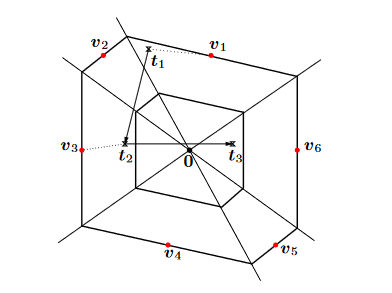
\includegraphics[width = 0.5\textwidth]{voronoi_cells.png}
    \caption{A graphical representation of the Voronoi cell \ac{CVP} algorithm \cite{10.1007/978-3-642-20901-7_10}.}
\end{figure}

Now, we must understand how to compute such a list $V$ efficiently. We first note that if our lattice is of only one dimension, then the $V$ is simply $\pm \mathbf{b}_1$, and so using this information, we can build up our list of relevant vectors by utilising the fact that if we know the relevant vectors of $\mathcal{L}(\{\mathbf{b}_1,...,\mathbf{b}_{n-1}\})$, we can easily search by exhaustion for $V$ of $\mathcal{L}(\{\mathbf{b}_1,...,\mathbf{b}_{n}\})$ as the extra relevant vectors will not be far, allowing us to bound our search.


\begin{algorithm}[H]
    \caption{Compute relevant vectors}
    \begin{algorithmic}[1]
    \State \textbf{Input:} Basis $\mathbf{B} = \{\mathbf{b}_1,...,\mathbf{b}_n\}$
    \State $\mathbf{B} \gets \mbox{LLL}(\mathbf{B})$
    \State $V_1 = \{\mathbf{b}_1, -\mathbf{b}_1\}$
    \For {$i \gets 2, n$}
        \State $V_i \gets \{\}$
        \State $\mathbf{B}_i \gets \{\mathbf{b}_1,...,\mathbf{b}_i\}$
        \For {$\mathbf{c} \in \{\{0,1\}^i \backslash \mathbf{0}\} $}
            \State $\mathbf{t} \gets -\frac{\mathbf{B}_i\mathbf{c}}{2}$
            \State $h_t \gets \frac{\left\langle \mathbf{t},\mathbf{b}^*_i\right\rangle }{|\mathbf{b}^*_i|^2}$
            \State $\mathbf{best} \gets \mbox{NearestPlaneCVP}(\mathbf{t}, \mathbf{B}_i)$
            \For {$h$ s.t. $|h - h_t| \cdot |\mathbf{b}^*_i| < |\mathbf{best}|$}
                \State $\mathbf{v} \gets \mbox{Alg.\ref{alg:CVP}}(\mathbf{t}-h\mathbf{b}_i, V_{i-1}) + h\mathbf{b}_i$
                \If{$|\mathbf{best}| < |\mathbf{v}|$}
                    \State $\mathbf{best} \gets \mathbf{v}$
                \EndIf
            \EndFor
            \State $V_i \gets V_i \cup \{\pm 2(\mathbf{best} - \mathbf{t})\}$
        \EndFor
        \For {$\mathbf{v}_j\in V_i$}
            \If{$\exists \mathbf{v}_n \in V_k : \mathbf{v}_n \neq \mathbf{v}_j, \left\lvert \frac{\mathbf{v}_j}{2} - \mathbf{v}_n\right\rvert  = \left\lvert \frac{\mathbf{v}_j}{2}\right\rvert$}
                \State $V_k \gets V_k \backslash \{\mathbf{v}_j-, -\mathbf{v}_j\}$
            \EndIf
        \EndFor
    \EndFor
    \State \textbf{return} $V_n$
    \end{algorithmic}
\end{algorithm}

It can be seen from this, that computing exact Voronoi cells can be computationally expensive, and so we can use approximate Voronoi cells, cutting down much of the computation.

\begin{figure}[h]
    \centering
    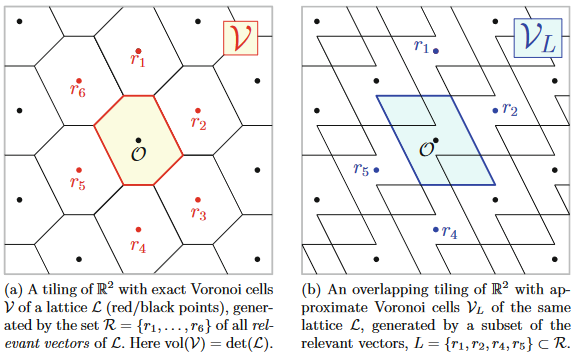
\includegraphics[width = 0.8\textwidth]{approx_voronoi.png}
    \caption{A graphical representation Voronoi cells against approximate voronoi cells \cite{10.1007/978-3-030-25510-7_1}.}
\end{figure}


\subsection{Dual Attack}

\begin{definition}[Dual lattice]
    Given a lattice $\mathcal{L}$, let $\mathcal{L} ^*$ be the corresponding dual lattice, where $\mathcal{L} ^*$ contains all vectors $\mathbf{v} \in span(\mathcal{L})$ such that $\langle \mathbf{v}, \mathbf{w} \rangle \in \mathbb{Z}$ for all $\mathbf{w} \in \mathcal{L}$. For a full rank lattice with basis $\mathbf{B}$, its dual is given by $\mathbf{B}^{-T}$.
\end{definition}

The dual attack relies on the following concept; given $(\mathbf{A, b}) \in (\mathbb{Z}/q\mathbb{Z})^{m \times n} \times (\mathbb{Z}/q\mathbb{Z})^m$, find many small vectors $v_i$ such that if our sample is an \ac{LWE} sample, we have $\langle \textbf{b, v}_i \rangle$ is also small, and is distributed according to a modular Gaussian distribution. If this is not the case, and our sample is random, then these values will be distributed randomly (and not necessarily small).

We can use this concept to develop an algorithm that allows us to enumerate the secret from a given \ac{LWE} sample. First, we must find many vectors $(\mathbf{x}_j, \mathbf{y}_j)$ in such a way that $\mathbf{x}_j^T\mathbf{A}=(\mathbf{y}^T_{j,1}||\mathbf{y}^T_{j,2})$ and $(\mathbf{x}_j, \mathbf{y}_{j,2})$ is short, where $\mathbf{y}_{j,1}$ and $\mathbf{y}_{j,2}$ is partitioned in the same way that we split $\mathbf{s}$ into two components, $\mathbf{s}_1$ and $\mathbf{s}_2$ such that $\mathbf{s}^T = (\mathbf{s}_1^T||\mathbf{s}_2^T)$, and similarly, $\mathbf{A}=(\mathbf{A}_1||\mathbf{A}_2)$ such that $\mathbf{b}=\mathbf{As+e}=\mathbf{A}_1 \mathbf{s}_1 + \mathbf{A}_2 \mathbf{s}_2 + \mathbf{e}$.

We are then able to notice that we may create a new sample, $(\mathbf{A}_2, \mathbf{b - A}_1 \bar{\mathbf{s}}_1)$, where $\bar{\mathbf{s}}_1$ is our guess for the first part of the secret. If our guess is correct, then this new sample will act like a genuine \ac{LWE} sample, and we can use the distinguishing methods we earlier described, and will describe this in more depth later.

\begin{algorithm}[H]
    \caption{Dual Attack in general}
    \begin{algorithmic}[1]
    \State \textbf{Input:} $(n,m,q,\chi _{\mathbf{s}}, \chi _{\mathbf{e}})$ LWE parameters, $k_1, k_2 \in \mathbb{Z}$ s.t. $k_1+k_2=n$, and $(\mathbf{A, b})\in (\mathbb{Z}/q\mathbb{Z})^{m \times n} \times (\mathbb{Z}/q\mathbb{Z})^m$ LWE pair.
    \State Find many vectors $(\mathbf{x}_j, \mathbf{y}_j)$ s.t. $\mathbf{x}_j^T\mathbf{A}=(\mathbf{y}_{j,1}^T|\mathbf{y}_{j,2}^T)$ and $(\mathbf{x}_j, \mathbf{y}_{j,2})$ are short. \Comment Finding these short vectors is usually done by reducing the lattice using \ac{BKZ} and sieving as the \ac{SVP} oracle. The output from the first block will normally suffice.
    \For{all possible $\tilde{\mathbf{s}}_1$ for $\mathbf{s}_1$}
        \State $X = \{(\mathbf{x}_j^T(\mathbf{b}-\mathbf{A}_1\tilde{\mathbf{s}}_1))|\forall \mathbf{x}_j\}$
        \If{$X\sim N$} \Comment As opposed to distributed uniformly.
            \State \textbf{return} $\tilde{\mathbf{s}}_1$
        \EndIf
    \EndFor
    \end{algorithmic}
\end{algorithm}

\newpage

\section{Algorithm specification of \textsc{Kyber}.PKE}

\textbf{Note:} We will present a simplified and abstracted version of the algorithm, for example, omitting `compress', `encode' and other such functions in order to more easily analyse the algorithm as opposed to it's implementation.

\textsc{Kyber}.\ac{PKE} is defined over the ring $R \equiv \mathbb{Z} /(X^n+1)$ and $R_q\equiv \mathbb{Z}_q[X]/(X^n+1)$ where $n=2^{n'-1}$ s.t. $X^{n}+1$ is the $2^{n'}$\textsuperscript{th} cyclotomic polynomial [citecrystals]. For this chapter, our notation will be slightly different, with regular upper and lowercase letters denoting elements in $R$ or $R_q$, and our notation for vectors instead denoting vectors with coefficients in $R$ or $R_q$. In relation to our earlier explained \ac{LWE} problem, $R$ is $\mathbb{F}$ and $R_q$ is $\mathbb{F}_q$. 

\subsection{Generate Keys}
We begin, by generating our matrix $\mathbf{A}$ using the following algorithm:
\begin{algorithm}[H]
    \caption{Generate keys.}
    \begin{algorithmic}[1]
    \State $N:=0$
    \State $(\rho, \sigma ):=G(d)$ \Comment Where G is a hash function s.t. $G:\mathcal{B}^* \rightarrow \mathcal{B}^{32}\times  \mathcal{B}^{32}$
    \For{$i\gets 0, k-1$}
        \For{$j\gets 0, k-1$}
            \State $\mathbf{A}:=Parse(XOF(\rho , j, i))$ \Comment This essentially generates a random $k\times k$ matrix over $R_q$ as $\rho$ is pseudorandom from the hash function $G()$.
        \EndFor
    \EndFor
    \For{$i\gets 0, k-1$}
        \State $\mathbf{s}:=CBD(PRF(\sigma ,N))$ \Comment Where CBD is a function outputting a polynomial in $R_q$ with the coefficients distributed central-binomially. $PRF$ is a pseudorandom function, $PRF:\mathcal{B}^{32} \times \mathcal{B} \rightarrow \mathcal{B}^*$.
        \State $N:=N+1$
    \EndFor
    \For{$i\gets 0, k-1$}
        \State $\mathbf{e}:=CBD(PRF(\sigma ,N))$
        \State $N:=N+1$
    \EndFor
    \State $\mathbf{s}:= NTT(\mathbf{s})$ \Comment Where \ac{NTT} is a bijection mapping $f \in R_q$ to a polynomial with the coefficient vector.
    \State $\mathbf{e}:= NTT(\mathbf{e})$
    \State $\mathbf{b}:=\mathbf{As}+\mathbf{e}$
    \State \textbf{return} $\mathbf{A}$, $\mathbf{s}$, $\mathbf{b}$, $\mathbf{e}$
    \end{algorithmic}
\end{algorithm}

From this, we have our public and private keys, $pk:=(\mathbf{b}\mod{q})\| \rho $ and $sk:=\mathbf{s}\mod{q}$ (both encoded).

\subsection{Encryption}

\begin{algorithm}[H]
    \caption{Encryption}
    \begin{algorithmic}[1]
    \State \textbf{Input:} $pk$, $m \in \mathcal{B}^{32}$
    \State first we must extract $\mathbf{A}$ and $\mathbf{b}$ from $pk$.
    \State $\rho:=pk+12\cdot k\cdot \frac{n}{8}$ \Comment $\rho$ was simply appended to the end of $\mathbf{b}$ so we can extract it simply. As we now have $\rho$ we can re-construct $\mathbf{A}$ like we did in key generation.
    \For{$i\gets 0, k-1$}
        \For{$j\gets 0, k-1$}
            \State $\mathbf{A}^T:=Parse(XOF(\rho , i, j))$ 
        \EndFor
    \EndFor
    \For{$i\gets 0, k-1$}
        \State $\mathbf{r}:=CBD(PRF(r ,N))$ \Comment Where $r \in \mathcal{B}^{32}$ is a random coin.
        \State $N:=N+1$
    \EndFor
    \For{$i\gets 0, k-1$}
        \State $\mathbf{e}_1:=CBD(PRF(r ,N))$
        \State $N:=N+1$
    \EndFor
    \State $e_2:=CBD(PRF(r, N))$
    \State $\mathbf{r}:=NTT(\mathbf(r))$
    \State $\mathbf{u}:=NTT^{-1}(\mathbf{A}^T\circ \mathbf{r})+\mathbf{e}_1$
    \State $v:=NTT^{-1}(\mathbf{b}^T\circ \mathbf{r})+e_2 + m $
    \State \textbf{return} $(\mathbf{u}\|v)$
    \end{algorithmic}
\end{algorithm}

It is important that the ciphertext composes of two parts, only one of which is dependent on the message, so that the receiver has enough information in order to decrypt correctly.

\subsection{Decryption}

\begin{algorithm}[H]
    \caption{Decryption}
    \begin{algorithmic}[1]
    \State \textbf{Input:} $sk$, $c$
    \State $m:=v-NTT^{-1}(\mathbf{s}^T\circ NTT(\mathbf{u}))$
    \State \textbf{return} $m$
    \end{algorithmic}
\end{algorithm}

It may not be readily obvious why it is this decryption works:
\begin{align*}
    v-NTT^{-1}(\mathbf{s}^T\circ NTT(\mathbf{u})) &= NTT^{-1}(\mathbf{b}^T\circ \mathbf{r}+e_2+m)-NTT^{-1}(\mathbf{s}^T\circ NTT(\mathbf{u}))\\
    &=NTT^{-1}(\mathbf{b}^T\circ \mathbf{r}+e_2+m)-NTT^{-1}(\mathbf{s}^T\circ \mathbf{A}^T\circ \mathbf{r}+\mathbf{e}_1)\\
    &=NTT^{-1}(\mathbf{b}^T\circ \mathbf{r}+e_2+m-\mathbf{s}^T\circ \mathbf{A}^T\circ \mathbf{r}+\mathbf{e}_1)\\
    &=NTT^{-1}(( \mathbf{A} \circ \mathbf{s})^T \circ \mathbf{r} - (\mathbf{s}^T \circ \mathbf{A} ^T) \circ \mathbf{r} + \mathbf{e} ^T + \mathbf{e}_1 + e_2 + m)\\
    &=NTT^{-1}(m+\mathbf{e}^T+\mathbf{e}_1+e_2)
\end{align*}

Therefore, we decrypt by rounding to the nearest $\lfloor c \cdot \frac{q}{32} \mod{q}\rfloor $ for some $c \in \mathbb{N}$.
% \section{Executive Summary}



\section{Applying our security notions to LWE and \textsc{Kyber}.PKE}

It can be seen that the security of \textsc{Kyber}.\ac{PKE} can be reduced to the hard problem of \ac{LWE}; in other words, given $LWE_{n,m,q,\chi _\mathbf{s}, \chi _\mathbf{e}}$ is hard then \textsc{Kyber}.\ac{PKE} is \ac{LWE}-\ac{CPA} secure. In both our security notions, we rely on the statement
\[\mathbb{P} (\mathcal{A} \mbox{ succeeds}) = 1/2 + \varepsilon \mbox{\qquad where $\varepsilon$ is negligible.}\]

and so we can define what $\mathbb{P} (\mathcal{A} \mbox{ succeeds})$ is in order to begin to analyse the security of \textsc{Kyber}.\ac{PKE}, and so we have $\mathbb{P} (\mathcal{A} \mbox{ succeeds})=$

\[\mathbb{P} (a =  i |\substack{ (pk, sk) \leftarrow \textsc{Kyber}.\ac{PKE}.KeyGen(),\\ (m_0, m_1) \leftarrow \mathcal{A}(pk),\\ c \leftarrow \textsc{Kyber}.\ac{PKE}.Enc(pk, m_i),\\ a \leftarrow \mathcal{A}(s, c)}) \qquad \mbox{for $i \in \{0,1\}$.}\]


Therefore, the advantage of the adversary (in our earlier definition written as $\varepsilon$),\\ $\mathbf{Adv}^{\ac{CPA}}_{\textsc{Kyber}.\ac{PKE}}(\mathcal{A}) =$
\[ |\mathbb{P} (a =  i |\substack{(pk, sk) \leftarrow \textsc{Kyber}.\ac{PKE}.KeyGen(),\\ (m_0, m_1) \leftarrow \mathcal{A}(pk),\\ c \leftarrow \textsc{Kyber}.\ac{PKE}.Enc(pk, m_i),\\ a \leftarrow \mathcal{A}(s, c)}) - \frac{1}{2}| \]

In other words, if $\mathbf{Adv}^{\ac{CPA}}_{\textsc{Kyber}.\ac{PKE}} \approx 0$ (or the adversary has no advantage), then \textsc{Kyber}.\ac{PKE} is \ac{CPA} secure.\par

We can also do the same thing for an \ac{LWE} problem, and define the advantage of our adversary over this problem. The \ac{LWE} challenge that our adversary must solve is slightly different to our challenge that we gave them for \textsc{Kyber}.\ac{PKE}, and instead of distinguishing which message created the challenge ciphertext, they must determine if the challenge was generated via the \ac{LWE} scheme, or if it was generated randomly. Thus, our $\mathbf{Adv}^{\ac{LWE}}(\mathcal{A})=$
\[ |\mathbb{P}(b'=1|\substack{\mathbf{A}\leftarrow R^{m\times k}_q,\\ (\mathbf{s, e}) \leftarrow \mathcal{B}^k \times \mathcal{B}^m,\\ \mathbf{b} = \mathbf{As+e},\\ b'\leftarrow \mathcal{A}(\mathbf{A,b})}) - \mathbb{P}(b'=1|\substack{\mathbf{A}\leftarrow R^{m\times k}_q ,\\\mathbf{b}\leftarrow R^m_q,\\ b'\leftarrow \mathcal{A}(\mathbf{A,b})})| \]

It can be seen that $\mathbf{Adv}^{\ac{CPA}}_{\textsc{Kyber}.\ac{PKE}}(\mathcal{A})$ can be re-written as:

\[ |\mathbb{P}(b'=1|\substack{\mathbf{A} \leftarrow R^{m\times k}_q ,\\ (\mathbf{s, e}) \leftarrow \{0, 1\}^k \times \{0,1\}^m ,\\ \mathbf{b} = \mathbf{As} + \mathbf{e} + m_i ,\\ a \leftarrow \mathcal{A}(\mathbf{A,b})}) - \frac{1}{2}| \]

by using the definitions of \textsc{Kyber}.\ac{PKE}'s algorithms. Thus, we can show that the \ac{IND}-\ac{CPA} security of \textsc{Kyber}.\ac{PKE} is reducible to that of the \ac{LWE} scheme, $\mathbf{Adv}^{\ac{LWE}}(\mathcal{A})\approx $
\[ |\mathbb{P}(b'=1|\substack{\mathbf{A} \leftarrow R^{m\times k}_q ,\\ (\mathbf{s, e}) \leftarrow \{0, 1\}^k \times \{0,1\}^m ,\\ \mathbf{b} = \mathbf{As} + \mathbf{e} + m_i ,\\ a \leftarrow \mathcal{A}(\mathbf{A,b})}) - \frac{1}{2}| \]

as $\mathbb{P}(b'=1|\substack{\mathbf{A}\leftarrow R^{m\times k}_q ,\\\mathbf{b}\leftarrow R^m_q,\\ b'\leftarrow \mathcal{A}(\mathbf{A,b})})|$ can simply be reduced to the expected value $\frac{1}{2}$.

\[ \Rightarrow \mathbf{Adv}^{\ac{CPA}}_{\textsc{Kyber}.\ac{PKE}}(\mathcal{A}) \leq_T \mathbf{Adv}^{\ac{LWE}}(\mathcal{A}) \]

\section{Tailoring the Dual Attack to \textsc{Kyber}}

MATZOV published a paper in which they detail improvements to the dual attack in order to further increase its efficacy at enumerating secrets \cite{matzov_2022_6412487}, something that proves very interesting for those interested in the security levels of \textsc{Kyber}. This comes largely through the use of \ac{FFT} during the distinguishing process, allowing us to check all values at once instead of one at a time, as well as improved methods to sample short vectors. The formal definition of the improved algorithm is as follows:


\begin{algorithm}[H]
    \caption{MATZOV Improved Dual Attack \cite{matzov_2022_6412487}}
    \begin{algorithmic}[1]
    \State \textbf{Input:} $(n,m,q,\chi _{\mathbf{s}}, \chi _{\mathbf{e}})$ LWE parameters, $\beta _1, \beta _2 \leq d$ where $\beta _1, \beta _2 \in \mathbb{Z}$, $k_{enum}, k_{fft}, k_{last}$ s.t. $k_{enum} + k_{fft} + k_{last} = n$, $p \in \mathbb{Z}$ s.t. $p \leq q$, $D \in \mathbb{Z}$, $C \in \mathbb{R}$, and $(\mathbf{A, b})\in (\mathbb{Z}/q\mathbb{Z})^{m \times n} \times (\mathbb{Z}/q\mathbb{Z})^m$ LWE pair.
    \State
    \State $\mathbf{A}_{last} := (\mathbf{a}_{n-k_{last}}...\mathbf{a}_n)$ \Comment The last $k_{last}$ columns of $\mathbf{A}$.
    \State $\alpha = \frac{\sigma _\mathbf{e}}{\sigma _\mathbf{s}}$
    \State $\mathbf{B} = 
        \begin{pmatrix}
            \alpha \mathbf{I}_m & 0\\
            \mathbf{A}^T_{last} & q \mathbf{I}_{k_{last}}
        \end{pmatrix}$
    \State $L = \mbox{shortVectors}(\mathbf{B}, \beta _1, \beta _2, D)$ \Comment Where $L$ is a list of D short vectors.
    \For{all possible $\bar{\mathbf{s}}_{enum}$} \Comment taken in decreasing order of probability according to $\chi _\mathbf{s}$.
        \State Let T be a table of dimension $p \times ... \times p$ ($k_{fft}$ times).
        \For{all short vectors $(\alpha \mathbf{x}_j, \mathbf{y}_{last}) \in L$}
        \State $\mathbf{y}_{j, fft} = \mathbf{x}^T_j \mathbf{A}_{fft}$
        \State $\mathbf{y}_{j, enum} = \mathbf{x}^T_j \mathbf{A}_{enum}$
        \State Add $e^{(\mathbf{x}^T_j\mathbf{b}-\mathbf{y}^T_{j, enum}\bar{\mathbf{s}}_{enum})\frac{2\pi i}{q}}$ to the $\left[\frac{p}{q}\mathbf{y}_{j, fft}\right]$th cell of T.
        \EndFor
    \State $\mbox{FFT}(T)$
    \If{$Re(\frac{1}{\psi (\bar{\mathbf{s}}_{fft})}T\left[\mathbf{s}_{fft}\right])>C$}
        \State \textbf{return} $\bar{\mathbf{s}}_{enum}$ \Comment Where $\psi (\bar{\mathbf{s}}_{fft})$ is a constant for centering our distribution.
    \EndIf
    \EndFor
    
    \end{algorithmic}
\end{algorithm}

\begin{algorithm}[H]
    \caption{Short Vectors \cite{matzov_2022_6412487}}
    \begin{algorithmic}[1]
    \State \textbf{Input:} Basis $\mathbf{B} = \{\mathbf{b}_1,...,\mathbf{b}_d\}$ for lattice $\mathcal{L}$, $D\in \mathbb{N}$, and $\beta _1, \beta _2 \in \mathbb{Z}$ s.t. $\beta _1, \beta _2 \leq d$
    \For {$i \gets 1, \left\lceil \frac{D}{N_{sieve}(\beta_2)} \right\rceil$} \Comment Where $N_{sieve}(d)$ is the number of vectors outputted by a sieving algorithm on a lattice of dimension $d$, and we are rounding with ties to rounding up.
        \State Randomise the basis $\mathbf{B}$
        \State Run \ac{BKZ} on our basis using blocksize $\beta_1$ on $\mathbf{B}$ to obtain a reduced basis $\mathbf{B}'$
        \State Run a sieving algorithm of dimension $\beta_2$ on the sublattice $\{\mathbf{b}'_1,...,\mathbf{b}'_{\beta_2}\}$ and add the outputted vectors to a list $H$.
    \EndFor
    \State \textbf{return} $H$
    \end{algorithmic}
\end{algorithm}

The lengths of these short vectors are at most:

\[\det (\mathcal{L})^{\frac{1}{d}}\cdot N_{sieve}(\beta _2)^{\frac{1}{\beta _2}}\cdot \sqrt{\frac{\beta_2}{2\pi e}\cdot(\pi \beta _2)^{\frac{1}{\beta _2}}}\cdot\delta(\beta_1)^{\frac{d-\beta_2}{2}}\]

Where $\delta(\beta_1) := \frac{|\mathbf{b}^*_i|}{|\mathbf{b}^*_{i+1}|}$ for the first $k<d-2\beta_1$ vectors of the Gram-Schmidt orthognalised basis.

The inputs to this algorithm are:
\begin{itemize}
    \item $D$: The number of short vectors to be found.
    \item $C$: The boundary by which guesses of the secret are judged.
    \item $\beta _1, \beta _2$: Parameters for $shortVectors$.
    \item $k_{enum}$: The number of secret coordinates we directly search.
    \item $k_{fft}$: The number of secret coordinates enumerated using \ac{FFT}.
    \item $k_{last}$: Remaining secrets.
    \item $p$: Modulus for FFT.
\end{itemize}

We also have $\mathbf{A, b}$ from an \ac{LWE} sample, where $\mathbf{s}$ and $mathbf{e}$ are sampled with known distributions $\chi _\mathbf{s}$ and $\chi _\mathbf{e}$ that have small variances $\sigma ^2_\mathbf{s}$ and $\sigma ^2_\mathbf{e}$ respectively. We then split $\mathbf{s}$ as dictated by our $k$ values, and also $\mathbf{A}$, thus giving us 
\[\mathbf{As} = \mathbf{A}_{enum}\mathbf{s}_{enum} + \mathbf{A}_{fft}\mathbf{s}_{fft} + \mathbf{A}_{last}\mathbf{s}_{last}\].

We can then find 
    \[B = \begin{pmatrix}
    \alpha \mathbf{I}_m & 0\\
    \mathbf{A}^T_{last} & q \mathbf{I}_{k_{last}}
\end{pmatrix}\]
where $\alpha = \frac{\sigma _\mathbf{e}}{\sigma _\mathbf{s}}$, and is only in place to account for the cases where $\chi _{\mathbf{s}} \neq \chi _{\mathbf{e}}$.

We can now use $shortVectors$ to find $D$ short vectors of $\mathbf{B}$, which can all be separated into the following form:

\[\mathbf{v} \equiv _q \begin{pmatrix}
\alpha \mathbf{x} \\
\mathbf{A}^T_{last}\mathbf{x}
\end{pmatrix}\]
and for each of these vectors 

\[\mathbf{x}^T\mathbf{b}=\mathbf{x}^T\mathbf{As}+\mathbf{x}^T\mathbf{e}.\]

Setting $\mathbf{y}^T = \mathbf{x}^T\mathbf{A}$, we can rewrite the above to give

\[\mathbf{x}^T\mathbf{b} = \mathbf{y}^T\mathbf{s} + \mathbf{x}^T\mathbf{e},\]

which when we split up $\mathbf{y}$ and $\mathbf{s}$ into the three constituent parts as described earlier, we have

\begin{align*}
    \mathbf{x}^T\mathbf{b} &= \mathbf{y}^T_{enum}\mathbf{s}_{enum} + \mathbf{y}^T_{fft}\mathbf{s}_{fft} + \mathbf{y}^T_{last}\mathbf{s}_{last} + \mathbf{x}^T\mathbf{e}\\ 
    \mathbf{y}^T_{enum}\mathbf{s}_{enum} + \mathbf{y}^T_{fft}\mathbf{s}_{fft} - \mathbf{x}^T\mathbf{b} &= -\mathbf{y}^T_{last}\mathbf{s}_{last} - \mathbf{x}^T\mathbf{e}
\end{align*}

Now, we apply the change of modulus by multiplying by $\frac{p}{q}$ and rounding the $y_{fft}$ component of our equation.

\[\frac{p}{q}\mathbf{y}^T_{enum}\mathbf{s}_{enum} + \frac{p}{q}\mathbf{y}^T_{fft}\mathbf{s}_{fft} - \frac{p}{q}\mathbf{x}^T\mathbf{b} = -\frac{p}{q}\mathbf{y}^T_{last}\mathbf{s}_{last} - \frac{p}{q}\mathbf{x}^T\mathbf{e}\]
\[\frac{p}{q}\mathbf{y}^T_{enum}\mathbf{s}_{enum} + (\left[\frac{p}{q}\mathbf{y}^T_{fft}\right]- \left[\frac{p}{q}\mathbf{y}^T_{fft}\right] + \frac{p}{q}\mathbf{y}^T_{fft})\mathbf{s}_{fft} - \frac{p}{q}\mathbf{x}^T\mathbf{b} = -\frac{p}{q}\mathbf{y}^T_{last}\mathbf{s}_{last} - \frac{p}{q}\mathbf{x}^T\mathbf{e}\]
\[\frac{p}{q}\mathbf{y}^T_{enum}\mathbf{s}_{enum} + \left[\frac{p}{q}\mathbf{y}^T_{fft}\right]\mathbf{s}_{fft} - \frac{p}{q}\mathbf{x}^T\mathbf{b} = -\frac{p}{q}\mathbf{y}^T_{last}\mathbf{s}_{last} - \frac{p}{q}\mathbf{x}^T\mathbf{e} - (\frac{p}{q}\mathbf{y}^T_{fft} - \left[\frac{p}{q}\mathbf{y}^T_{fft}\right])\mathbf{s}_{fft}\]

The right hand side of this expression is approximately distributed with modular Gaussian distribution, and so if we have the correct guesses, $(\bar{\mathbf{s}}_{enum}, \bar{\mathbf{s}}_{fft}) = (\mathbf{s}_{enum}, \mathbf{s}_{fft})$, then 

\[\frac{p}{q}\mathbf{y}^T_{enum}\bar{\mathbf{s}}_{enum} + \left[\frac{p}{q}\mathbf{y}^T_{fft}\right]\bar{\mathbf{s}}_{fft} - \frac{p}{q}\mathbf{x}^T\mathbf{b}\]

will also be distributed with a modular Gaussian distribution, whilst if not, it will be distributed uniformly. Finally, we must distinguish between those with the correct distribution, and so let us consider the below expression.

\[\mbox{FFT}((\bar{\mathbf{s}}_{enum}, \bar{\mathbf{s}}_{fft})) = Re(\frac{1}{\psi (\bar{\mathbf{s}}_{fft})}\sum_j e^{(\frac{p}{q}\mathbf{y}^T_{j,enum}\bar{\mathbf{s}}_{enum} + \left[\frac{p}{q}\mathbf{y}^T_{j,fft}\right]\bar{\mathbf{s}}_{fft} - \frac{p}{q}\mathbf{x}^T_j\mathbf{b})\frac{2\pi i}{p}})\]

where $\psi (\bar{\mathbf{s}}_{fft}) = e^{\frac{2\pi i c}{p}\sum_t\mathbf{s}_t}$, then if this value is approximately zero, our guess $\bar{\mathbf{s}}_{enum}$ is incorrect, and if above the cutoff $C$, then $\bar{\mathbf{s}}_{enum} = \mathbf{s}_{enum}$ (with overwhelming probability)\footnote{The higher our value for $C$, the more likely our guess is correct.}.

Let us write $\bar{\mathbf{s}}_{enum}$ as $\mathbf{s}_{enum} + \Delta \mathbf{s}_{enum}$, and $\bar{\mathbf{s}}_{ftt}$ as $\mathbf{s}_{ftt} + \Delta \mathbf{s}_{ftt}$ to give

\[\mbox{FFT}((\bar{\mathbf{s}}_{enum}, \bar{\mathbf{s}}_{fft})) = \sum_j Re(\frac{1}{\psi (\bar{\mathbf{s}}_{fft})}e^{(\frac{p}{q}\mathbf{y}^T_{j, enum}(\mathbf{s}_{enum} + \Delta \mathbf{s}_{enum}) + \left[\frac{p}{q}\mathbf{y}^T_{j, fft}\right](\mathbf{s}_{ftt} + \Delta \mathbf{s}_{ftt}) - \frac{p}{q}\mathbf{x}^T\mathbf{b})\frac{2\pi i}{p}})\]

Let us first assume that our guess is incorrect, in other words$\Delta \mathbf{s}_{enum}$ and $\Delta \mathbf{s}_{ftt}$ are non-zero.


\[\mbox{FFT}((\bar{\mathbf{s}}_{enum}, \bar{\mathbf{s}}_{fft})) = \sum_j Re(\frac{1}{\psi (\bar{\mathbf{s}}_{fft})}e^{(\frac{p}{q}\mathbf{y}^T_{j, enum}(\mathbf{s}_{enum} + \Delta \mathbf{s}_{enum}) + \left[\frac{p}{q}\mathbf{y}^T_{j, fft}\right](\mathbf{s}_{ftt} + \Delta \mathbf{s}_{ftt}) - \frac{p}{q}\mathbf{x}^T\mathbf{b})\frac{2\pi i}{p}})\]
    
\[= \sum_j Re(\frac{1}{\psi (\bar{\mathbf{s}}_{fft})}e^{\frac{p}{q}\mathbf{y}^T_{j,enum}\mathbf{s}_{enum} + \left[\frac{p}{q}\mathbf{y}^T_{j,fft}\right]\mathbf{s}_{fft} - \frac{p}{q}\mathbf{x}^T\mathbf{b} + \frac{p}{q}\mathbf{y}^T_{j,enum}\Delta\mathbf{s}_{enum} + \left[\frac{p}{q}\mathbf{y}^T_{j, fft}\right]\Delta \mathbf{s}_{fft}}\]

\[= \sum_j Re(\frac{1}{\psi (\bar{\mathbf{s}}_{fft})}e^{-\mathbf{y}^T_{j,enum}\Delta\mathbf{s}_{enum}\frac{2\pi i}{q}}e^{(\frac{p}{q}\mathbf{y}^T_{last}\mathbf{s}_{last} + \frac{p}{q}\mathbf{x}^T\mathbf{e} + (\frac{p}{q}\mathbf{y}^T_{j,fft} - \left[\frac{p}{q}\mathbf{y}^T_{fft}\right])\mathbf{s}_{fft} - \left[\frac{p}{q}\mathbf{y}^T_{j, fft}\right]\Delta \mathbf{s}_{fft})\frac{2\pi i}{q}})\]

Then, as the vectors $\mathbf{y}_{j, last}, \mathbf{y}_{j,enum}, \mathbf{y}_{j,fft},\mathbf{x}_j$ are independent, with $\mathbf{y}_{j,enum}, \mathbf{y}_{j,fft}$ distributed uniformly, and $/mathbf{y}_{j, last}, \mathbf{x}_j$ normally distributed around $0$, we can rewrite the second exponential and beginning reciprocal in terms of a new distribution:

\[\sum_j Re(e^{-\mathbf{y}^T_{j,enum}\Delta\mathbf{s}_{enum}\frac{2\pi i}{q}}e^{2\pi i W_j}\]

Where 

\[\mathbb{E} (\sum_j Re(e^{-\mathbf{y}^T_{j,enum}\Delta\mathbf{s}_{enum}\frac{2\pi i}{q}}e^{2\pi i W_j}) = 0\]

Now, assume that our guess is correct.

\[\mbox{FFT}((\bar{\mathbf{s}}_{enum}, \bar{\mathbf{s}}_{fft})) = \sum_j Re(\frac{1}{\psi (\bar{\mathbf{s}}_{fft})}e^{(\frac{p}{q}\mathbf{y}^T_{j, enum}(\mathbf{s}_{enum} + \Delta \mathbf{s}_{enum}) + \left[\frac{p}{q}\mathbf{y}^T_{j, fft}\right](\mathbf{s}_{ftt} + \Delta \mathbf{s}_{ftt}) - \frac{p}{q}\mathbf{x}^T\mathbf{b})\frac{2\pi i}{p}})\]

\[=\mbox{FFT}((\mathbf{s}_{enum}, \mathbf{s}_{fft})) = \sum_j Re(\frac{1}{\psi (\bar{\mathbf{s}}_{fft})}e^{(\frac{p}{q}\mathbf{y}^T_{j,last}\mathbf{s}_{last} + \frac{p}{q}\mathbf{x}^T_j\mathbf{e}+(\frac{p}{q}\mathbf{y}^T_{j,fft} - \left[\frac{p}{q}\mathbf{y}^T_{j,fft}\right])\mathbf{s}_{fft})\frac{2\pi i}{p}}\]

Where again, we can split this into parts of similar distribution to get

\[\sum_j Re(\varepsilon _{j,eq} \cdot \varepsilon_{j,round})\]

Which, when $D$ is sufficiently large, will be approximately normally distributed; the proofs for the mean and variance are too long and not particularly relevant to our goals in this paper and so are omitted. Using this, we have therefore found the first $k_{enum}$ digits of the key, and we can repeat the algorithm lengthening the portion of the key we are guessing whilst using the already enumerated part.

\newpage

\subsection{Impact on \textsc{Kyber}}

Below is verbatim the results presented by MATZOV \cite{matzov_2022_6412487} for interest of the reader.

\begin{figure}[H]
    \centering
    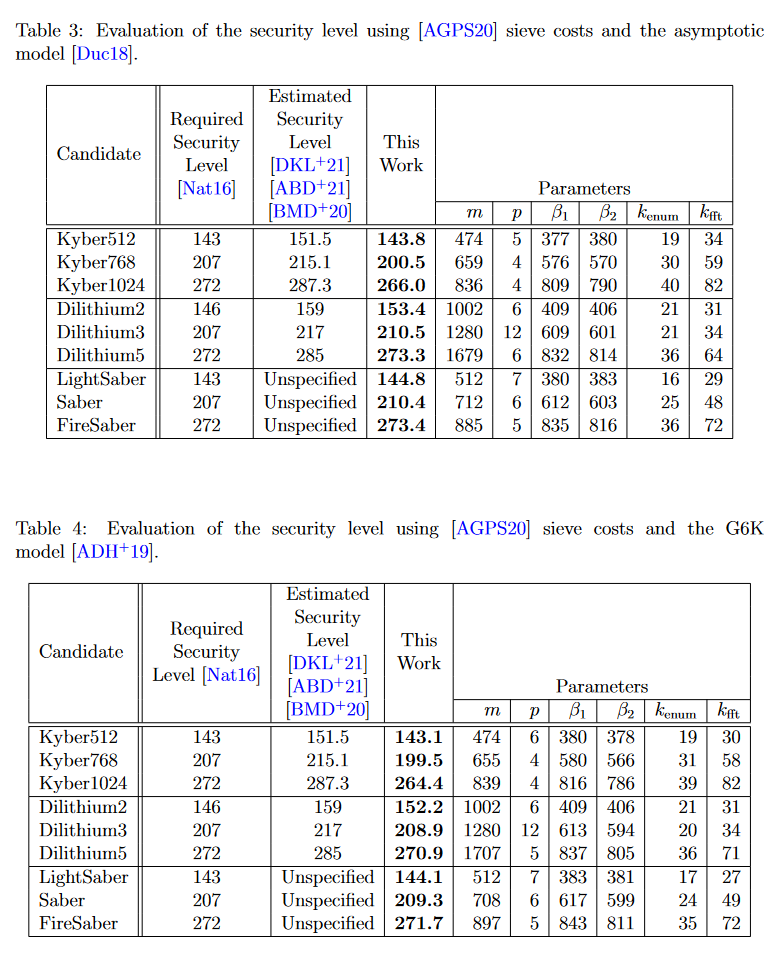
\includegraphics[width=0.8\textwidth]{matzov_results_1.png}
\end{figure}

\begin{figure}[H]
    \centering
    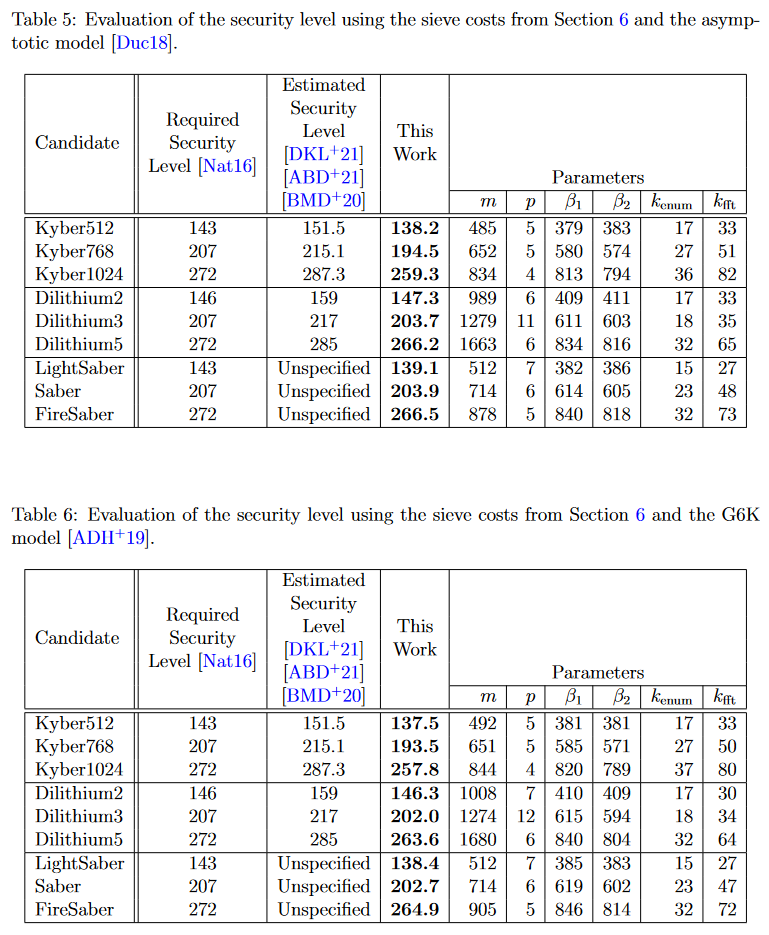
\includegraphics[width=0.8\textwidth]{matzov_results_2.png}
\end{figure}

\begin{figure}[H]
    \centering
    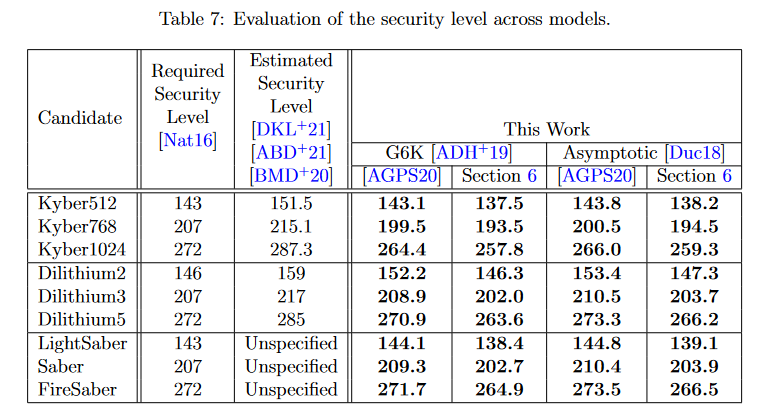
\includegraphics[width=0.8\textwidth]{matzov_results_3.png}
\end{figure}

\newpage

\section{Open Questions}
\textit{``To simplify the analysis, we do not assume the recovery of $\mathbf{s}_{fft}$. Although the above sum is expected to have large real value when $\mathbf{s}_{fft}$ is guessed correctly, it may also be large for certain wrong guesses of $\mathbf{s}_{fft}$, provided $\mathbf{s}_{enum}$ is guessed correctly. This does not concern us since we only wish to recover $\mathbf{s}_{enum}$."} \cite{matzov_2022_6412487}


This is possibly the most interesting paragraph of the whole MATZOV paper, and opens up the question; is it possible to distinguish between a wrong $\mathbf{s}_{fft}$ and a correct $\mathbf{s}_{fft}$, given that $\mathbf{s}_{enum}$ is correct? If so, it is likely that this would greatly increase the efficacy of the attack due to the fact we must use $p^k$ guesses.

We can also see that our fully constructed and tailored dual attack still relies on earlier mentioned techniques, specifically the use of sieving and the \ac{BKZ} algorithm when generating our list of small vectors. Due to the fact that our second use of sieving must return all found short lattice vectors, we are unable to utilise `dimensions-for-free' \cite{inbook}, however, is there a method by which we can manipulate the lattice used for this in order to allow us to utilise such technique? Alternatively, any improvements of sieving algorithms or \ac{BKZ} is likely to increase the potency of this dual attack. Also, is it possible to implement pre-processing somewhere in this attack? Perhaps the same techniques we use when utilising Voronoi cells can be implemented elsewhere, and on the topic of Voronoi cells, can we reduce the space required by somehow compressing our requirements of Voronoi cells - approximate Voronoi cells, and generally how to choose the parameters, such that our cells are accurate enough yet still much easier to compute.

More generally, however, the ideal choice for a lot of variables - such as how many bits we should enumerate at one time, and $\beta_1, \beta_2$ - is yet to be fully solved. For example, it can be seen that by reducing the number of bits we are enumerating, we decrease our search space for that run but in doing so we reduce the potential advantage we are aiming to achieve over simply guessing by brute force.

\newpage
\nocite{*}
\printbibliography
\end{document}